\begin{tikzpicture}[
    x=1cm,
    y=1cm,
    stage/.style={
        draw,
        rounded corners=2pt,
        semithick,
        align=center,
        minimum height=11mm,
        text width=32mm,
        fill=gray!8
    },
    transform/.style={
        draw,
        rounded corners=2pt,
        semithick,
        align=center,
        minimum height=11mm,
        text width=32mm,
        fill=gray!8
    },
    snippetstage/.style={
        draw,
        line width=0.35pt,
        draw=black!30,
        minimum width=37mm,
        minimum height=24mm,
        fill=white
    },
    smstage/.style={
        draw,
        line width=0.35pt,
        draw=black!30,
        minimum width=37mm,
        minimum height=24mm,
        fill=white
    },
    component/.style={
        draw,
        rounded corners=2pt,
        line width=0.35pt,
        draw=black!35,
        align=center,
        minimum height=10mm,
        text width=34mm,
        fill=gray!8
    },
    support/.style={
        draw,
        rounded corners=2pt,
        semithick,
        align=center,
        minimum height=11mm,
        text width=37mm,
        fill=blue!10
    },
    test/.style={
        draw,
        rounded corners=2pt,
        semithick,
        align=center,
        minimum height=11mm,
        text width=37mm,
        fill=green!12
    },
    result/.style={
        draw,
        rounded corners=2pt,
        line width=0.35pt,
        draw=black!35,
        align=center,
        minimum height=10mm,
        text width=34mm,
        fill=orange!14
    },
    note/.style={
        align=center,
        font=\small,
        text width=38mm
    },
    resultlabel/.style={
        align=center,
        font=\small
    },
    flow/.style={->, semithick},
    attach/.style={->, dashed, semithick}
]

\node[snippetstage] (source) at (0,0) {};
\node[transform] (driver) at (4.4,0) {драйвер\\компилятора};
\node[transform, text width=38mm] (language) at (8.6,0) {лексический и\\синтаксический\\анализ};
\node[smstage] (stack) at (13.1,0) {};

\node[anchor=north west, inner sep=0pt] at ($(source.north west)+(0.8mm,-0.8mm)$) {
    \begin{tikzpicture}[x=1mm,y=-1mm]
        \clip (0,0) rectangle (36.4,21.9);
        \node[
            anchor=north west,
            align=left,
            font=\ttfamily\fontsize{4.6}{5.1}\selectfont
        ] at (0.05,0.05)
            {var x, y, z;\\
             \\
             fun zip (x) \{\\
             \ \ case x of Pair (x, y) ->\\
             \ \ \ \ case x of\\
             \ \ \ \ \ \ Nil          ->  Nil\\
             \ \ \ \ | Cons (x, xs) -> case y of\\
             \ \ \ \ \ \ \ \ \ \ \ \ \ \ \ Nil ->  Nil\\
             \ \ \ \ \ \ \ \ \ \ \ \ \ \ | Cons (y, ys) ->\\
             \ \ \ \ \ \ \ \ \ \ \ \ \ \ \ \ Cons (Pair (x, y),\\
             \ \ \ \ \ \ \ \ \ \ \ \ \ \ \ \ \ \ zip (Pair (xs, ys)))\\
             \ \ \ \ \ \ \ \ \ \ \ \ \ \ esac\\
             \ \ \ \ esac};
        \node[anchor=south east, font=\ttfamily\tiny, text=gray!65]
            at (36.8,21.5) {$\ddots$};
    \end{tikzpicture}
};
\node[font=\small, align=center, below=1mm of source] {исходная\\программа};

\node[anchor=north west, inner sep=0pt] at ($(stack.north west)+(0.8mm,-0.8mm)$) {
    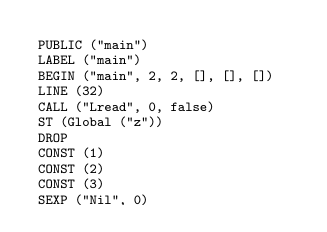
\begin{tikzpicture}[x=1mm,y=-1mm]
        \clip (0,0) rectangle (34.4,22.4);
        \node[
            anchor=north west,
            align=left,
            font=\ttfamily\fontsize{5.0}{5.6}\selectfont
        ] at (0.1,0.25)
            {PUBLIC ("main")\\
             LABEL ("main")\\
             BEGIN ("main", 2, 2, [], [], [])\\
             LINE (32)\\
             CALL ("Lread", 0, false)\\
             ST (Global ("z"))\\
             DROP\\
             CONST (1)\\
             CONST (2)\\
             CONST (3)\\
             SEXP ("Nil", 0)\\
             SEXP ("Cons", 2)};
    \end{tikzpicture}
};

\node[component] (native-backend) at (13.1,2.7) {нативная\\генерация кода};
\node[resultlabel] (native-code) at (17.2,2.7) {нативный код};
\node[support, fill=gray!12, text width=32mm] (execenv) at (15.2,4.4) {среда выполнения};
\node[support, fill=gray!12, text width=32mm] (stdlib) at (19.2,4.4) {стандартная\\библиотека};

\node[resultlabel] (bytecode) at (17.2,0) {байткод};
\node[resultlabel] (stackinterp) at (13.1,-2.8) {интерпретация\\стекового представления};
\node[resultlabel] (sourceinterp) at (8.6,-2.8) {интерпретация\\исходного языка};

% \node[test, text width=34mm] (tests) at (4.4,2.7) {регрессионные\\тесты};

\draw[flow] (source) -- (driver);
\draw[flow] (driver) -- (language);
\draw[flow] (language) -- (stack);

\draw[flow] (stack) -- (native-backend);
\draw[flow] (native-backend) -- (native-code);
\draw[flow] (stack) -- (bytecode);
\draw[flow] (stack) -- (stackinterp);
\draw[flow] (language) -- (sourceinterp);

\draw[attach]   (native-code) -- (execenv);
\draw[attach]  (native-code) -- (stdlib);
% \draw[attach] (tests) -- (driver);

\end{tikzpicture}
